\documentclass{article}
\usepackage[utf8]{inputenc}
\usepackage{graphicx}
\usepackage{subfig}
\usepackage[margin=0.75in]{geometry}

\begin{document}
	\begin{center}
    
		\LARGE{\textbf{Automatic Path Planning for Agricultural Irrigation Vehicles}} \\
        \vspace{1em}
        \normalsize\textbf{Yunfeng Xin, Zhengyu Chen, Feng Chen} \\
        \vspace{1em}
        \large{Project Proposal} \\
        \vspace{1em}
     
	\end{center}
    \begin{normalsize}
    
    	\section{Motivation:}
        
            Coverage Path Planning(CPP) is a well-studied topic in recent years. Different approaches is applied to solve this type of problem including A* search\cite{b1}, dynamic programming \cite{b2}and neutral network\cite{b3}. Luis Piardi\cite{b4} suggested using Q-learning to optimize CPP, however, the result turned to involve unnecessary turns in the path planning. An increasing number of turns is inefficient for agricultural vehicles since it introduced more acceleration and deceleration in the real-world application. In this project, we will model this problem as a Markov Decision Process(MDPs) and solve it by using reinforcement learning. The goal for this project is to find an optimal complete coverage path with a relatively fewer number of turns. 
      
		\section{Problem Definition:}
		
		    \subsection{Data Inputs and Outputs:}
		    
		        The input to our path planning system will be a graph describing the landscape that requires irrigation. To simplify our problem, the graph will be discrete and contains connected blocks. The graph has a starting block indicating the initial position of the agent, an exiting block indicating the final position the agent must reach after completing the irrigation, and positions of the obstacles which the agent needs to avoid. The agent will try to traverse the graph with the least travelling distance. Additionally, we want to impose real-world constraints such as requiring the least number of turns because it is costly for agricultural vehicles to make a turn. Finally, the agent will output an episode of actions indicating a path from the start to the end point.
		        
            \begin{figure}[htp]
                \centering
                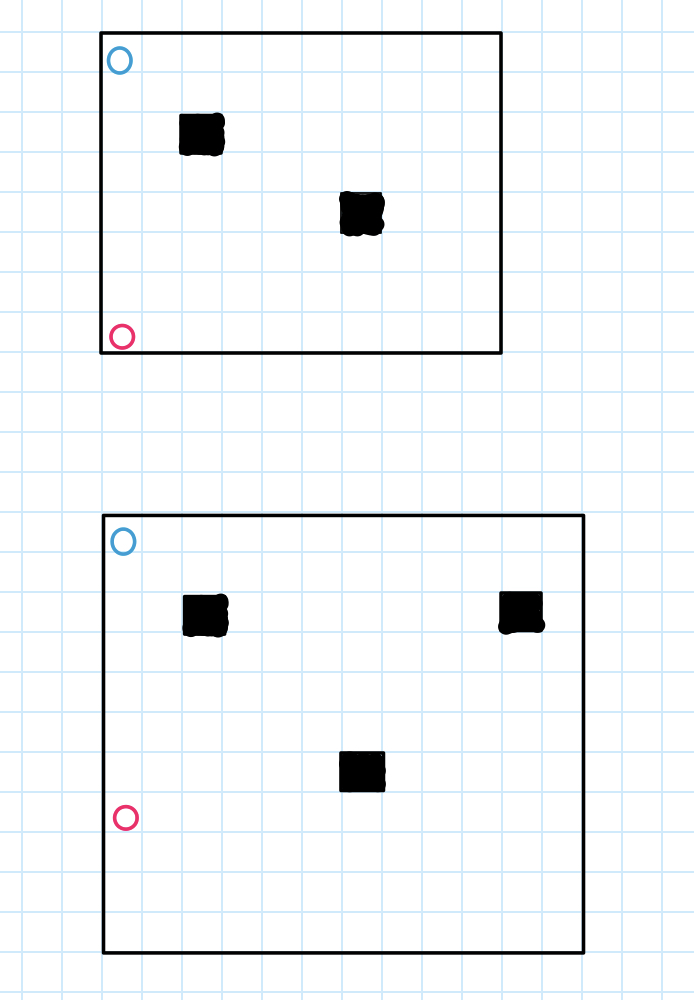
\includegraphics[width=3.5cm]{IMG_2619.jpg}
                \qquad
                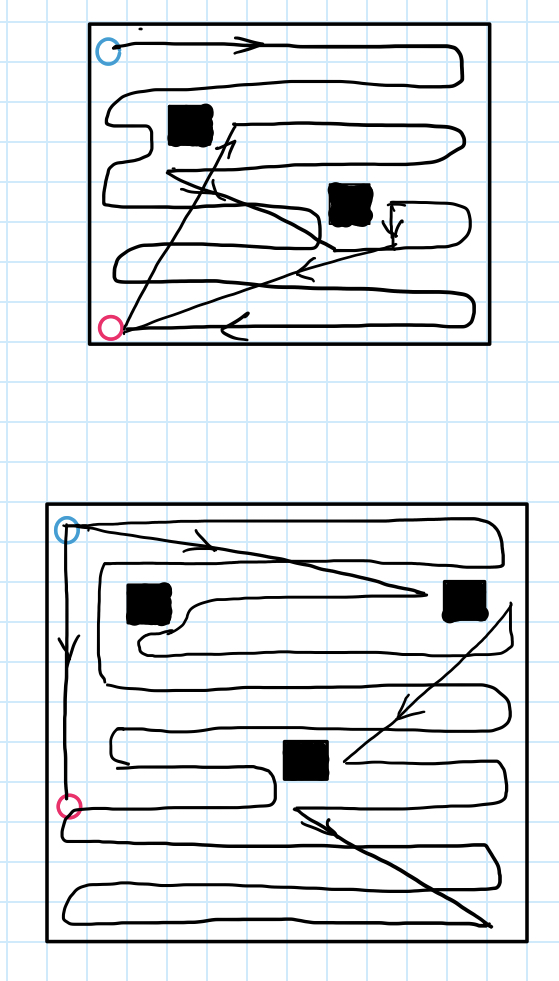
\includegraphics[width=3.5cm]{IMG_2620.jpg}
                \caption{Sample input(left) and output(right), blue circle refer to starting block, red circle refer to exiting block}
            \end{figure}

		        
		    \subsection{Baseline and Oracle:}
		    
		        Since we allow agents to repeatedly visit a block which is the case in our real world, we plan to set our baseline to an agent that always goes to the nearest block that is not irrigated. If multiple candidate blocks are available, it will randomly pick among these blocks. \par 
		        
		        Under our minimal travelling distance constraint, the oracle will be a human trying to traverse all the blocks in the graph without visiting repeated blocks. However, this is infeasible in most of the situations, and even a human needs to go through a trial and error process, and won't be sure if the final solution is optimal. Additionally, if we impose other constraints such as requiring the least number of turns, the problems becomes even less intuitive. \par
		        
		        The gap between the oracle and the baseline is due to the fact that greedy algorithms such as the baseline cannot take possible future states into account, while a typical human has some level of intuition about what might be a good choice of route in order to traverse the entire graph (i.e. going straight until a obstacle or boundary is met).
            
        \section{Method:}
            
            \subsection{Challenges:}
            
                There are a few challenges of the project. The first challenge is to model the real process. The reward of the total distance, total number of turns, total time used need to be carefully evaluated so that our model will reflect the real world problems. The second challenge is whether AI algorithms will be trapped in local minimums (or maximums), which prevents finding the optimal strategy. The third challenge is how well our learned strategy will generalize to problems with extra constrains such as barricades. Last but not least, the state space in the CPP problem is quite large. So how to use the neural network to extract the features and perform the best is a challenge.
                
            \subsection{Approach:}
            
                The approach of this project is reinforcement learning (RL). As we don't know the Markov decision process (MDP) and our goal is not to learn the MDP, we will choose model-free RL algorithms. If we don't want to loose any information, the state of the problem will be all the past tracks. Suppose a 2D graph with $N \times N$ blocks and only consider 4 ways of turning, the total number of states is on the order of $4^{N^2}$. With such a large state space, we turn to deep reinforcement learning. The idea is to use deep neural network (DNN) to help generalize state features. RL updating algorithms will then applied to learn the weights and the policies. As there may be large correlations between the policies of nearby states, convolutional neural network (CNN) will be helpful. Moreover, if we want to generalize our model to continuous actions (e.g. continuous turning angle), we may need to switch to more sophisticated algorithms such as Deep Deterministic Policy Gradient (DDPG).
            
            \subsection{Evaluation Metrics:}
            
                The optimal path planning should provide a route which minimized the total travel time and fully cover the field without unnecessary repeated visit.
                Total travel time can be estimated by set the operation speed for going straight and the turning speed for turns. (i.e., operation speed $>$ turning speed) Our team plan to evaluate the performance of our agent based on several metrics including the total travel time, the percentage of coverage and the percentage of repeated visit. We will compare the outputs from agents with different policies to the outputs of our baseline as well as several attempts of the same problem from a real human. We will also assign multiple sets of weights to these evaluation metrics to see if different weights will affect these decisions. 
                
            
        \section{Social impact:}
        
        This project is aimed to find an optimal strategy for CPP, which can be applied to the agricultural irrigation fields. In the real world, the landscape can be complex and it is almost impossible for us to optimize the path planning manually. Thus, if using AI to solve CPP is feasible, the efficiency of automatic irrigation will be improved, which will have great economic and environmental benefits.  Moreover, this project can be easily developed for different real world applications like cleaning robots, underwater mining, etc. 
        
    \end{normalsize}
  
  \newpage
    \begin{thebibliography}{00}
        \bibitem{b1}A. Ntawumenyikizaba, Hoang Huu Viet and TaeChoong Chung, "An online complete coverage algorithm for cleaning robots based on boustrophedon motions and A* search," 2012 8th International Conference on Information Science and Digital Content Technology (ICIDT2012), Jeju, 2012, pp. 401-405.
        \bibitem{b2}Peng Zhou and Zhong-min Wang and Zhen-nan Li and Yang Li, "Complete Coverage Path Planning of Mobile Robot Based on Dynamic Programming Algorithm", 2nd International Conference on Electronic \& Mechanical Engineering and Information Technology, 2012
        \bibitem{b3}Galceran, Enric, and Marc Carreras. "A survey on coverage path planning for robotics." Robotics and Autonomous systems 61.12 (2013): 1258-1276.
        \bibitem{b4}Luis Piardi, José Lima, Ana I. Pereira, and Paulo Costa. "Coverage path planning optimization based
        on Q-learning algorithm"AIP Conference Proceedings 2116, 220002 (2019)
        
    \end{thebibliography}
    
\end{document}
